%\documentclass[12pt,openany,oneside,a4paper,english,brazil]{abntbibufjf}
\documentclass[preprint,12pt]{elsarticle}

\usepackage{lmodern}
\usepackage[T1]{fontenc}
\usepackage[utf8]{inputenc}		%% Para converter automaticamente acentos como digitados. Mude utf8 para latin1 se precisar.
                                        %% Permite digitar os acentos no teclado normalmente, sem comandos (\'e \`a , etc.).
\usepackage{lastpage}
\usepackage{indentfirst}
\usepackage{color}
\usepackage{graphicx}
\usepackage{microtype}
\usepackage{floatrow}

%% -----------------------------------------------------------------------------

%% Obs.: Alguns acentos foram omitidos.

%\titulo{Uma ferramenta para recomendação de revisores de código para apoiar a colaboração em Desenvolvimento Distribuído de Software} %%Por exemplo, Titulo da tese
\title{Uma ferramenta para recomendação de revisores de código para apoiar a colaboração em Desenvolvimento Distribuído de Software}
\journal{None}

% \subtitulo{: subt\'itulo do trabalho}  %% Retirar o primeiro ``%'' desta linha se for utilizar subtitulo. Deixar os dois pontos antes, em ``: subt\'itulo'' .
%\autor{Vinicius Junqueira Schettino}
%\autorR{Junqueira Schettino, Vinicius} %%Colocar o sobrenome do autor antes do primeiro nome do autor, separados por ,

\author{Vinicius Schettino}
\address{Federal University of Juiz de Fora - Brazil }



%\local{Juiz de Fora}
%\data{2018} %%Alterar o ano se precisar
%\orientador[Orientador:]{Marco Antônio Pereira Araújo} %%Se precisar, troque [Orientador:] por [Orientadora:]
% \coorientador[Coorientador:]{Nome do coorientador } %% Retirar o primeiro ``%'' desta linha se tiver coorientador. Se precisar, troque por [Cooorientadora:].
%\instituicao{Universidade Federal de Juiz de Fora}
%\faculdade{Instituto de Ciências Exatas} %%Alterar, dentro de chaves {}, se precisar.
%\programa{Programa de Pós-graduação em Ciência da Computação} %%Alterar, dentro de chaves {}, se precisar.
%\objeto{Dissertação (Mestrado)}  %%Tese (Doutorado)
%\natureza{Dissertação apresentada ao \insereprograma ~da Universidade Federal de Juiz de Fora, como requisito parcial para obtenção do título de Mestre em Ciência da Computação.}


%% Abaixo, prencher com os dados da parte final da ficha catalografica

%\finalcatalog{1. Palavra-chave. 2. Palavra-chave. 3. Palavra-chave. I. Pereira Araújo, Marco Antônio, orient. II. T\'itulo.} %% Aqui fica
% escrito a palavra ``T\'itulo'' mesmo, nao o do trabalho. Se tiver coorientador, os dados ficam depois dos dados
%% do orientador (II. Sobrenome, Nome do coorientador, coorient.) e antes de ``II. T\'itulo'', o qual passa a ``III. T\'itulo''.

%% ---

%\setlength{\parindent}{1.3cm}

%\setlength{\parskip}{0.2cm}

%\setlength\afterchapskip{12pt}


%% Iniciar o documento
\begin{document}
\begin{frontmatter}

%% ELEMENTOS PRE-TEXTUAIS

%% Capa
%\inserecapa

%% Folha de rosto
%\inserefolhaderosto


%% Ficha catalografica. AO IMPRIMIR, DEIXAR NO VERSO DA FOLHA DE ROSTO.
%\inserecatalog


%% Folha de aprovacao
%\begin{folhadeaprovacao}

%  \begin{center}
%    {\chapterfont \bfseries \insereautor}

%    \vfill
%    \begin{center}
%      {\chapterfont\bfseries\inseretitulo \inseresubtitulo}
%    \end{center}
%    \vfill

%    \hspace{.45\textwidth}
%    \begin{minipage}{.5\textwidth}
%        \inserenatureza
%    \end{minipage}%
%    \vfill
%   \end{center}

%   Aprovada em: %%COLOCAR A DATA

%   \begin{center} BANCA EXAMINADORA \end{center}
%   \assinatura{Prof. Dr. \insereorientador \ - Orientador \\ Universidade Federal de Juiz de Fora}
%  \assinatura{Professor Dr. \inserecoorientador \ - Coorientador \\ Universidade Federal de Juiz de Fora}
%   \assinatura{Professor Dr. ?? \\ Universidade ???}
%   \assinatura{Professor Dr. ?? \\ Universidade ??}
%  \assinatura{...} %%RETIRE O % E PREENCHA SE PRECISAR
%  \assinatura{...}
%  \assinatura{...}
%\end{folhadeaprovacao}


%% Dedicatoria. OPCIONAL. Retirar o ``%'' de cada das 4 linhas abaixo, caso queira.
% \begin{dedicatoria} \vspace*{\fill} \centering \noindent
%   \textit{ Dedico este trabalho ... (opcional)}
%   \vspace*{\fill}
% \end{dedicatoria}


%% Agradecimentos. OPCIONAL. CASO SEJA BOLSISTA, INSERIR OS DEVIDOS AGRADECIMENTOS.
%\begin{agradecimentos}

%De acordo com a Associa\c{c}\~ao Brasileira de Normas T\'ecnicas - 14724 (2011, p. 1) Agradecimentos
%\'e o ``texto em que o autor faz agradecimentos dirigidos \`aqueles que contribu\'iram de maneira relevante \`a elabora\c{c}\~ao %do trabalho.''

%\end{agradecimentos}

%% Epigrafe. OPCIONAL
%\begin{epigrafe}
%    \vspace*{\fill}
%	\begin{flushright}
%		``Texto em que o autor apresenta uma cita\c{c}\~ao, seguida de autoria, relacionada com a
%mat\'eria tratada no corpo do trabalho'' \\
%(ASSOCIA\c{C}\~AO BRASILEIRA DE NORMAS T\'ECNICAS, 2011, p. 2) \\
%A ep\'igrafe elaborada conforme NBR 10520 (Ep\'igrafe - Opcional)
	\end{flushright}
\end{epigrafe}


%% RESUMOS

%% Resumo em Portugu^es. OBRIGATORIO.
%\setlength{\absparsep}{18pt}
%\begin{resumo}
%De acordo com a Associa\c{c}\~ao Brasileira de Normas T\'ecnicas - 6028 (2003, p. 2) ``o resumo deve ressaltar
%o objetivo, m\'etodo e as conclus\~oes do documento (...) Deve ser composto de uma sequ\^encia de frases
%concisas, afirmativas e n\~ao de enumera\c{c}\~ao de t\'opicos. Recomenda-se o uso de par\'agrafo \'unico.''
%O resumo deve ter de 150 a 500 palavras.

%Palavras-chave: Palavra-chave. Palavra-chave. Palavra-chave. %finalizadas por ponto e inicializadas por letra maiuscula.

%\end{resumo}

\begin{abstract}

\end{abstract}

%% Resumo em Ingle^s
%\begin{resumo}[ABSTRACT]
% \begin{otherlanguage*}{english}
% ...
\end{frontmatter}

%Key-words: ...
% \end{otherlanguage*}
%\end{resumo}

%% Seguindo o mesmo modelo acima, pode-se inserir resumos em outras linguas.

%% Lista de ilustracoes. OPCIONAL.
%\pdfbookmark[0]{\listfigurename}{lof}
%\listoffigures*
%\cleardoublepage


%% Lista de tabelas. OPCIONAL. Retire o ``%'' de cada das 3 linhas seguintes, caso queira.
% \pdfbookmark[0]{\listtablename}{lot}
% \listoftables*
% \cleardoublepage

%% Lista de abreviaturas e siglas. OPCIONAL
%\begin{siglas} %%ALTERAR OS EXEMPLOS ABAIXO, CONFORME A NECESSIDADE%
%  \item[UFJF] Universidade Federal de Juiz de Fora
%  \item[DDS]  Desenvolvimento Distribuído de Software
%\end{siglas}

%% Sumario
%\pdfbookmark[0]{\contentsname}{toc}
%\tableofcontents*
%\cleardoublepage

%% ----------------------------------------------------------

%% ELEMENTOS TEXTUAIS

%\textual
%\pagestyle{simple}


\chapter{INTRODUÇÃO}  %%Nesta linha, dentro de { }, digita-se em CAIXA ALTA, como apresentado aqui

  O \textit{code review} é considerado uma das principais técnicas para diminuição de defeitos de software \cite{Boehm2001}. Nela, o autor de uma alteração na base de código de um projeto submete tal conteúdo ao crivo de um conjunto de pares técnicos, que irão revisar sua estrutura com base em um lista de regras e convenções previamente definida. Diferentes aspectos relacionados ao autor, ao revisor e ao processo de revisão em si estão diretamente relacionados à eficiência da prática. Autores relatam relação da diminuição da incidência de \textit{anti-patterns} \cite{Kemerer2009} de acordo com o nível de participação dos envolvidos e cobertura do código revisado \cite{Meneely201437, Morales2015171, Bavota201581}. Reputação \cite{Baysal2013122, Bosu2014} e experiência \cite{Kononenko2015111} do revisor também parecem impactar nos efeitos do \textit{code review}

  Intrinsecamente colaborativa, a atividade hoje é exercida com suporte de ferramentas computacionais específicas \cite{Bacchelli2013}, principalmente no desenvolvimento distribuído. Dentro de workflows de trabalho descentralizados \cite{gousios2016}, a prática funciona como um \textit{gateway} de qualidade que busca garantir que apenas alterações aderentes aos padrões de qualidade do projeto serão incorporados à codebase principal. Esta etapa do desenvolvimento se torna uma oportunidade para disseminação de conhecimento, embate de ideias e discussão de melhores práticas entre profissionais de experiência e visões diferentes.

  Tais aspectos configuram o Desenvolvimento Distribuído de Software (DDS), onde equipes de desenvolvimento se encontram espalhadas por organizações e espaços geográficos distintos. Este novo ramo da Engenharia de Software vem modificando a relação entre empresas e sistemas, principalmente em relação às estratégias de negócios \cite{audy2007}. As próprias relações de negócios fomentam a distribuição das equipes, procurando diminuição dos custos e a incorporação de mão de obra qualificada que pode estar em qualquer lugar do planeta.

  Neste contexto, porém, os os desafios à colaboração co-localizada são potencializados e as soluções tradicionais não são suficientes para fomentar esta aspecto das atividades distribuídas \cite{nicolaci2011}. Casey \cite{casey2010} mostra que, com a distribuição geográfica dos times, diversos outros desafios, antes considerados colaterais ou resolvidos, emergem de forma a ameaçar a colaboração entre os membros da equipe: barreiras culturais, temporais e geográficas; reengenharia dos processos de desenvolvimento; resistência em compartilhar informações e conhecimento com os pares distribuídos; entre outros desafios.

  Estes desafios do Desenvolvimento Distribuído de Software afetam o \textit{code review} de duas formas distintas. Primeiro, o processo de revisão pode se tornar lento e ineficiente quando a colaboração é afetada, devido aos baixos níveis de participação e cobertura. O mesmo vale para a disseminação do conhecimento, que fica prejudicada. Outro desafio que se consolida é a escolha do revisor adequado para aquele \textit{patch}. Com um vasto número de opções e pouca informação disponível sobre seus aspectos técnicos e gerenciais (e.g. tempo disponível) já que não há contato co-localizado entre eles, a natureza distribuída deste tipo de desenvolvimento dificulta o processo de escolha do revisor, impactando negativamente a eficiência do processo.

  Uma possível solução, visando amparar o desafio da colaboração e evitando o \textit{overhead} da escolha do revisor, seria manter grupos bem testados e experientes exercendo as atividades de revisão. Ou ainda, fixar, dentro de cada equipe de desenvolvimento, quem são os responsáveis por revisão e pela submissão dos \textit{patches}, evitando a diversificação das relações de trabalho.

  Contudo, estudos recentes demonstram que a fixação de grupos e responsabilidades pode não ser benéfica para o processo de desenvolvimento. Scott Page \cite{page2008} argumenta que a diversidade de experiências, visões e especilidades fazem com que grupos sejam mais eficientes. Já Prikladnicki et al. \cite{prikladnicki2017} apontam índicios de que a formação de grupos temporários em detrimento ou em conjunto com permanentes é um fator de eficiência em projeots de software:

  \begin{description}
    ``Although old colleagues bring knowledge of the development process and prior norms from previous teams, new members bring fresh ideas that could promote project performance and creativity. Old colleagues might not do so and might not give new members a chance to implement their ideas.''
  \end{description}

  Essa visão aponta que a formação  dinâmica dos grupos de trabalho em desenvolvimento de software potencializa a disseminação do conhecimento, um dos objetivos primários do \textit{code review} \cite{Bacchelli2013}.

  Existem alguns trabalhos congêneres que demonstram métodos de recomendação de revisores. Esses trabalhos foram estudados e levados em consideração para escrita do presente texto. Também foram revisadas pesquisas que apontam caracterísitcas de revisões, revisores e autores que possivelmente potencializam a colaboração. Tais aspectos são apresentados e discutidos no capítulo~\ref{chap:trabalhos_relacionados}.

  As principais lacunas deixadas pelos trabalhos anteriores estão relacionadas aos objetivos e à avaliação dos métodos propostos, principalmente em DDS. Primeiramente, não há relato de método de recomendação de revisores de código com o objetivo específico de potencializar a colaboração. Por isso, métodos já propostos não utilizam métricas nem variáveis de entrada relacionadas aos aspectos de cooperação, coordenação e comunicação, como por exemplo a abordagem 3C em DDS \cite{fuks2003}. Neste modelo, proposto por Ellis et al. \cite{ellis1991} em 1991 utiliza estas três dimensões para analisar a capacidade que sistemas têm de propiciar a colaboração para trabalhos em grupo.

  A segunda lacuna é observável na avaliação dos modelos de avaliação. Os trabalhos encontrados se limitam a comparar seus resultados com métricas relacionadas à proximidade dos mesmos com a indicação manual do revisor. Ou seja, a eficência é tida de acordo com a interseção entre o recomendado automaticamente e por decisão de um especialista, geralmente um desenvolvedor. Este modelo assume que o responsável pela indicação manual tem os subsídios naturais para fazer uma boa escolha. Em DDS isso pode não ser verdade, uma vez que fatores como diferenças culturais, de horário, geográficas e de maturidade podem diminuir a compreensão do indicador e propiciar a escolha inadequada do revisor. Por isso, no contexto apresentado, outras formas de avaliação podem ser mais apropriadas. Tais discussão são extendidas no capítulo~\ref{chap:metodos}}.

  Expostos os desafios que o Desenvolvimento Distribuído de Software impõe sobre a escolha do revisor de código, a importância da indicação do revisor adequado do ponto de vista de colaboração e a motivação da formação de grupos heterogêneos e dinâmicos, sumariza-se o intuito do presente texto. De acordo com a abordagem QGM (Goal/Question/Metric) proposta por Basili et al. \cite{Basili1984}, postula-se o objetivo do trabalho como:  \textbf{Implementar} um método de recomendação de revisores \textbf{com o objetivo de} potencializar a colaboração \textbf{em relação aos aspectos} de coordenação \textbf{do ponto de vista} de revisores e autores \textbf{no contexto de} desenvolvimento distribuído de software.

  A principal hipótese que norteia o andamento desta proposta, e que será revisitada e discutida nos capítulos derradeiros é:

  \begin{itemize}
    \item O método de recomendação apresentado pode potencializar a colaboração entre revisores e autores.
  \end{itemize}

  O uso de ferramentas computacionais para o processo de revisão de código se tornou prática comum nos últimos anos \cite{Bacchelli2013}. O GitHub, possivelmente a maior plataforma de código do planeta, é uma plataforma rica em repositórios de projetos de software. Muitos são de código aberto, disponíveis para mineração. Discussões sobre o \textit{workflow} de trabalho na ferramenta em contraponto à métodos tradicionais de revisão podem ser vistas na seção~\ref{sec:code_review}. São 24 milhões de usuários, 67 milhões de projetos e 47 milhões de revisões\footnote{https://octoverse.github.com/}, também chamadas de \textit{pull requests} no modelo de desenvolvimento ``\textit{pull based}'' \cite{gousios2014}. Essa abordagem é explorada em pormenores na seção~\ref{sec:pull_based}.

  Esta característica permitiu a extração e análise automatizadas das informações sobre as revisões em projetos de código aberto, através de APIs disponibilizadas para este fim. Foram as extraídas métricas apontadas como relevantes para nossos objetivos pela literatura relacionada. A arquitetura que embasa a extração e análise destes dados com objetivo de recomendação é explicada no capítulo~\ref{chap:solucao}.

  A avaliação da eficiência do método proposto apresenta particularidades em relação à trabalhos relacionados, devido ao enfoque em colaboração no contexto de DDS. O método de avaliação é devidamente discutido e aplicado no capítulo~\ref{chap:resultados}, incluindo a apresentação dos experimentos e a revisitação da hipótese levantada neste capítulo. Por fim, o capítulo~\ref{chap:conclusao} é dedicado ao fechamento do trabalho, inclusindo a sugestação de trabalhos futuros e a discussão de ameaças a validade e generalização dos resultados apresentados.


\chapter{PRESSUPOSTOS TEÓRICOS}\label{chap:metodos}

  \section{\textit{Code review}}\label{sec:code_review}
    O \textit{code review} é uma prática consolidade e difundida em diversas organizações, contemplando diferentes portes e segmentos de mercado. A técnica constitui da análise técnica de uma mudança a ser submetida à base principal de código (repositório-mestre) por parte de um revisor técnico, tendo como base uma lista de diretrizes e padrões a serem observados. As nuances do processo variam em cada contexto, levando em consideração por exemplo tolerância a defeitos, modelo de desenvolvimento e os objetivos almejados.

  \subsection{Relevância}\label{sec:relevancia}
    O \textit{code review} está associada diretamente à detecção precoce de defeitos em produtos de software \cite{schettino2014,Kemerer2009}, sendo reconhecida como uma das princpais técnicas com este fim \cite{Boehm2001}. Mais especificamente, é relatada maior eficiência quanto aos defeitos não-funcionais, enquanto os defeitos funcionais são menos afetados no processo \cite{Beller2014202}. Outros autores reportam a diminuição de defeitos através de estudos de caso \cite{McIntosh2014192,Bavota201581,Morales2015171}.

  \subsection{Histórico}\label{sec:historico}
    A atividade de revisão remonta da décade de 80 \cite{Fagan1976}, e desde então vem evoluindo para suportar interações mais rápidas e constantes, com uso de ferramentas computacionais e práticas ágeis. O Modern Code Review (MCR) surge em sinergia com os modelos ágeis e distribuídos de desenvolvimento, valorizando mais a comunicação e troca de experiências entre autor e revisor \cite{Bacchelli2013}.

  \subsection{Pull Based Method}\label{sec:pull_based}
    O conceito de \textit{branches} é a base para sistemas de controle de versão descentralizados, como o  Git\footnote{https://git-scm.com/} e o Mercurial\footnote{https://www.mercurial-scm.org/}. Com as \textit{branches} é possível desenvolver paralelamente, submtendo e mesclando as alteraçoẽs no código em momentos oportunos. Esta característica é interessante para o DDS, uma vez que o isolamento e a atomicidade do trabalho de cada um até o momento de submissão é fundamental para a coordenação dos esforços \cite{barr2012}.

    Estas tecnologias permitiram o surgimento de um paradigma de desenvolvimento baseado em pulls, ou \textit{pull-based method} \cite{gousios2014}. O processo de revisão de código evolui neste novo paradigma, servindo como um \textit{gateway} de qualidade que busca garantir que apenas alterações aderentes aos padrões de qualidade do projeto serão incorporados à codebase principal \cite{gousios2015}. A figura~\ref{fig:pull-request-flow} ilustra tal modelo de trabalho instanciado no GitHub\footnote{https://github.com}, principal expoente que oferece este paradigma. Nele é representado um modelo comum em desenvolvimento OpenSource \cite{6385140}, onde há um \textit{core team} responsável por revisar os \textit{pulls} de seus colegas e da comunidade no geral. Neste modelo, a mudança chega à codebase principal somente se houver o aval de um membro do \textit{core team}.

     \begin{figure}[!htbp]
      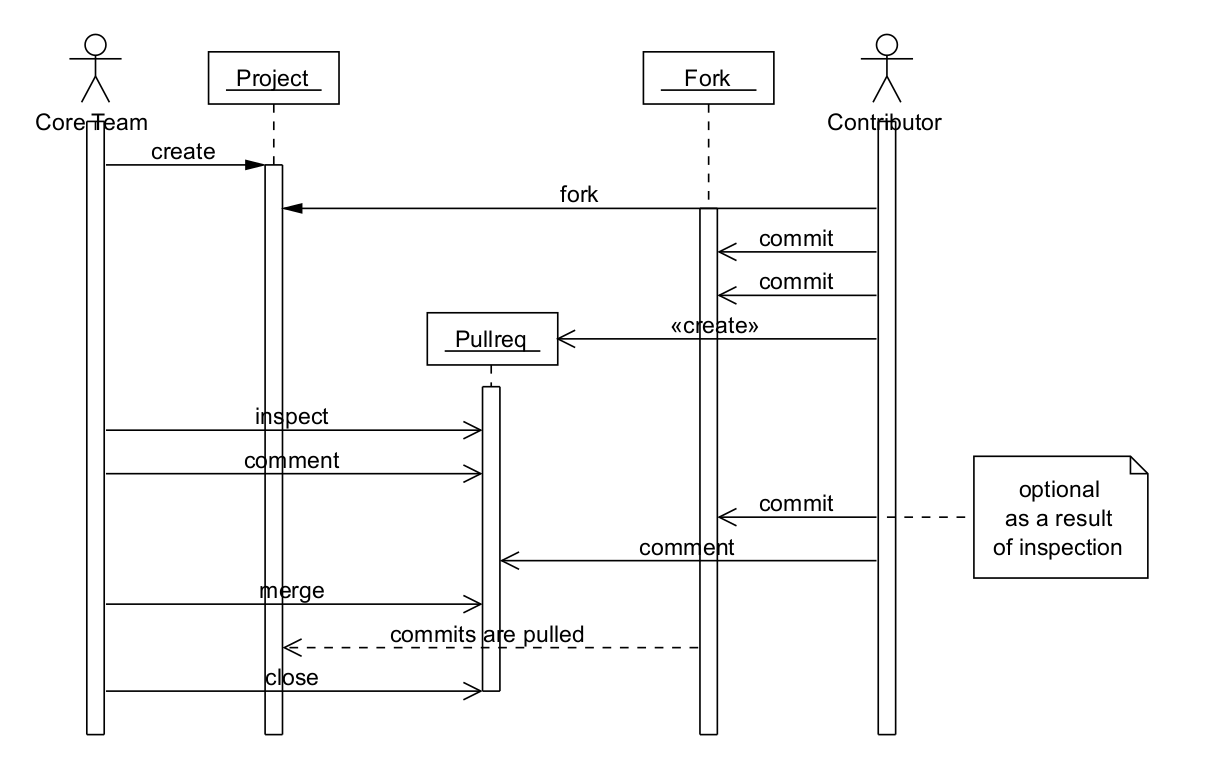
\includegraphics[width=\textwidth]{pull-request-flow}\label{fig:pull-request-flow}
      \caption{Pull Request Process \cite{gousios2014}}
    \end{figure}

    O contribuidor cria para si uma cópia do projeto através de um \textit{fork}. Esta ação cria em seu diretório de trabalho um projeto idêntico ao original, mas onde ele tem acesso total de submissão e modificação. Nessa cópia, ele executa as modificações desejadas, geralmente em uma \textit{branch} dedicada para tal \cite{gousios2016}. Ao terminar, ele solicita a integração da \texit{branch} do \textit{fork} de volta ao projeto original. Essa solitação é chamada de \textit{pull-request}, que será analisada por um desenvolvedor com as devidas permissões. Durante esta revisão, o autor pode gerar novas modificações, geralmente atreladas aos pedidos do revisor. Ao final, a mudança é rejeitada (\textit{closed}) ou aceita \textit{merged}.

    Os membros do core também tem suas \textit{branches} revisadas por um processo análogo \cite{6385140,Bosu2014}. A principal diferença é que não há necessidade do \texit{fork}, já que eles tem as permissões necessárias para criar uma nova \textit{branch} no projeto-alvo.

  \section{Modelo 3c}\label{sec:modelo_3c}

  \section{Desenvolvimento Distribuído de Software}\label{sec:dds}


\chapter{REFERENCIAL TEÓRICO}\label{chap:trabalhos_relacionados}

  \section{Revisão sistemática da literatura}\label{sec:revisao_sistematica}

  \section{Métricas para recomendação do revisor}\label{sec:metricas_revisor}

  \section{Métricas de avaliação dos resultados}\label{sec:metricas_resultados}

  \section{Outros trabalhos relevantes}\label{sec:outros_trabalhos}



\chapter{SOLUÇÃO DESENVOLVIDA}\label{chap:solucao}
    (explicações técnicas, MER, tecnologias, etc)

\chapter{AVALIAÇÃO DA SOLUÇÃO}\label{chap:resultados}

  \section{Processo de Avaliação}

  \section{Apresentação dos resultados}\label{section:apresentacao}

  \section{Discussão dos resultados}\label{section:discussao}

\chapter{CONCLUSÃO}\label{chap:conclusao}

  \section{Ameaças}\label{section:ameacas}

  \section{Trabalhos futuros}\label{section:trabalhos_futuros}

  \section{Considerações finais}\label{section:consideracoes_finais}




%% ----------------------------------------------------------

%% ELEMENTOS POS-TEXTUAIS

\postextual

\bibliographystyle{elsarticle-num}
\bibliography{../bibrefs/refs.bib}




%% Apendices

\begin{apendicesenv}

\chapter{Artigo Mapeamento Sistemático}

Colocar aqui o artigo.


\begin{anexosenv}


\end{anexosenv}

%%% ---
\end{document}
\endinput
